\documentclass[10pt]{article} % For LaTeX2e
\usepackage{tmlr}
% Anonymous review configuration: do NOT use [accepted] or [preprint].

% Optional math commands from the official TMLR template package.
\input{math_commands.tex}

\usepackage{amsmath,amssymb,amsthm}
\usepackage{graphicx}
\usepackage{booktabs}
\usepackage{array}
\usepackage{multirow}
\usepackage{xcolor}
\usepackage{float}
\usepackage{algorithm}
\usepackage{algpseudocode}
\usepackage{microtype}

\usepackage{hyperref}
\usepackage{url}

\hypersetup{
    pdftitle={When Attention Repairs Itself: A Mechanistic Study of Backup Heads in GPT-2},
    pdfauthor={Anonymous},
    pdfsubject={Mechanistic Interpretability of Transformer Attention Circuits},
    pdfkeywords={mechanistic interpretability, Hydra Effect, self-repair, attention circuits, softmax normalization, causal intervention, Indirect Object Identification, GPT-2},
    pdfcreator={Anonymous},
    pdfproducer={Anonymous},
    colorlinks=true,
    linkcolor=blue!70!black,
    citecolor=blue!70!black,
    urlcolor=blue!70!black
}

\title{When Attention Repairs Itself: A Mechanistic Study of Backup Heads in GPT-2%
\thanks{Large language models, including an AI-assisted code editor, were used
as assistive tools during research planning, code development and review,
and manuscript editing. The authors independently verified the experimental
procedures, numerical results, citations, interpretations, and claims and take
full responsibility for the submitted work.}}

% Authors are hidden under the anonymous TMLR review option.
% Real author information is stored outside this submission package.
\author{\name Anonymous Author \email anonymous@submission.invalid \\
      \addr Anonymous Institution}

\def\month{MM}
\def\year{YYYY}
\def\openreview{\url{https://openreview.net/forum?id=XXXX}}

% Compact float/paragraph spacing (local to this submission; does not edit tmlr.sty).
\setlength{\parskip}{0.28pc}
\setlength{\textfloatsep}{6pt plus 1pt minus 2pt}
\setlength{\floatsep}{5pt plus 1pt minus 1pt}
\setlength{\intextsep}{6pt plus 1pt minus 2pt}
\setlength{\abovecaptionskip}{3pt}
\setlength{\belowcaptionskip}{1pt}
\setlength{\abovedisplayskip}{5pt plus 1pt minus 3pt}
\setlength{\belowdisplayskip}{5pt plus 1pt minus 3pt}
\setlength{\abovedisplayshortskip}{0pt plus 2pt}
\setlength{\belowdisplayshortskip}{3pt plus 1pt minus 2pt}
\setcounter{topnumber}{5}
\setcounter{bottomnumber}{4}
\setcounter{totalnumber}{8}
\renewcommand{\topfraction}{0.95}
\renewcommand{\bottomfraction}{0.9}
\renewcommand{\textfraction}{0.05}
\renewcommand{\floatpagefraction}{0.9}

\begin{document}

\maketitle

\begin{abstract}
A persistent ambiguity in mechanistic interpretability research concerns the
causal origin of the \emph{Hydra Effect}, the observed increase in attention
allocated by downstream ``backup'' attention heads to a target token after the
ablation of functionally dominant ``primary'' heads. The prevailing hypothesis
posits that this spike may be, at least in part, a passive mathematical artifact:
removing primary-head contributions collapses signal variance in the residual stream,
which triggers LayerNorm scaling changes. These LayerNorm-induced changes can raise
a target token's attention probability when competing logits shift downward or
shift less favorably. Disentangling this passive denominator effect from target-directed pre-softmax logit
changes has remained methodologically elusive under standard causal tracing.
We introduce the \textbf{Frozen Attention Logit Intervention}, a surgical
counterfactual technique that isolates the dynamic, ablation-induced pre-softmax
logit of a single target token while simultaneously freezing all non-target
pre-softmax logits to their clean-run baseline values. This construction
eliminates the confound of background denominator inflation, yielding a
counterfactual attention probability that reflects target-logit attention contributions.
We apply this method to GPT-2 Small \citep{radford2019language} on a cohort of
200 Indirect Object Identification (IOI) prompts \citep{wang2022interpretability},
evaluating all 144 attention heads across 12 layers.
Our principal finding is that in GPT-2 Small on a 200-example mixed-template
IOI cohort, ablating L9H9 and L10H0 induces a robust L10H10 increase in IO-directed
attention. This effect survives zero, mean, and resample ablation controls.
Path-stable FALI/Shapley decomposition shows that the attention increase is
dominated by the IO-target attention-logit contribution, while background-logit
changes oppose the spike on average. QK decomposition suggests the IO-target score
increase is primarily query-driven and largely cosine-alignment-driven.
Output mediation shows that the L10H10 attention-pattern change causally contributes
to IO-S logit recovery under this intervention, explaining about 43.6\% of
L10H10's zero-ablation degradation by aggregate ratio of means. We keep this
evidence separate from the LayerNorm-scale freezing diagnostic, which shows that under
the Layer-10 clean-scale intervention, 24.3\% of the observed L10H10 attention spike is removed
(reducing L10H10's attention delta from $+0.1893$ to $+0.1433$). While these results provide evidence for target-logit-specific compensatory routing in the GPT-2 Small IOI circuit under L9H9/L10H0 ablation, we bound our claims to this specific architecture, task, and intervention setup. Further work is required to determine whether similar backup mechanisms appear across broader model families and computational benchmarks.
\end{abstract}

\textbf{Keywords:} mechanistic interpretability, Hydra Effect, self-repair,
attention circuits, softmax normalization, causal intervention, Indirect Object
Identification, GPT-2, TransformerLens.

% ===================================================================
\section{Introduction}
\label{sec:intro}
% ===================================================================

The field of mechanistic interpretability seeks to reverse-engineer the
computational algorithms implemented by large language models (LLMs) at the
level of individual components, including attention heads, MLP neurons, and residual
stream directions \citep{elhage2021mathematical, olah2020zoom}. A central
research methodology is \emph{activation ablation}: nullifying or replacing the
output of a specific component and observing the cascade of effects on model
behavior. This approach has been instrumental in identifying the circuits
responsible for concrete capabilities, including Indirect Object Identification
\citep{wang2022interpretability}, modular arithmetic \citep{nanda2023progress},
and in-context learning \citep{olsson2022context}.

A well-documented but poorly understood phenomenon arising from ablation
experiments is the \textbf{Hydra Effect} \citep{mcgrath2023hydra}: the
systematic increase in attention weights that downstream ``backup'' heads
allocate to the ablated primary head's target token. This compensatory behavior
superficially resembles functional redundancy, where downstream backup heads exhibit
increased output to the target token under primary-head ablation. However, the mechanistic
origin of this spike is ambiguous.
Two competing explanations coexist:

\begin{enumerate}
  \item \textbf{Target-Directed Routing:} Under primary-head ablation, backup heads may increase the target-token relevance signal through changes in their query-key interactions, producing higher attention weights toward the target token.
  
  \item \textbf{Passive Softmax Denominator Shift (PSDS):} Ablating a primary
    head reduces the cumulative residual stream contribution to all downstream
    layers. This triggers a LayerNorm-mediated volume surge: the collapsed signal
    variance causes the normalization scale factor to inflate, which raises the
    pre-softmax logit magnitude of all tokens. Specifically, LayerNorm-induced changes can raise a target token's attention probability when competing logits shift downward or shift less favorably, even without any change in the underlying query-key alignment.
\end{enumerate}

Distinguishing target-logit changes from background-logit and denominator effects is critical for accurate circuit analysis. If the Hydra spike is predominantly a softmax or normalization artifact, then standard ablation experiments may overestimate the functional role of backup heads. Conversely, if the spike reflects target-directed pre-softmax logit changes, then post-softmax attention metrics can obscure the magnitude of the target-specific contribution.

Recent work has expanded both the empirical evidence for self-repair and the
methodological standards used to validate mechanistic explanations.
\citet{rushing2024selfrepair} demonstrate imperfect and prompt-dependent
self-repair across multiple language-model families and identify changes in
the final LayerNorm scaling factor and sparse anti-erasure neurons as
contributing mechanisms. More recently, \citet{gong2026conditional} introduce
Conditional Co-Ablation, an output-grounded method for recovering components
whose importance becomes visible only after a primary component set is
removed. Their experiments include backup-head recovery in the GPT-2 Small
IOI circuit and transfer to induction settings. These studies establish that
normalization effects and conditionally activated backups can confound
component attribution, but they do not present the target-token versus
competing-background pre-softmax decomposition studied here.

Prior circuit-discovery and path-patching methods
\citep{conmy2023automated,goldowsky2023localizing} provide causal tools for
localizing model behavior, but they do not directly isolate how a responsive
head's post-softmax attention change divides between its target-token logit and
the collection of non-target logits. FALI addresses this narrower
methodological gap by decomposing those contributions at the pre-softmax level
and relating the resulting attention-logit change to downstream causal
recovery. Work on the Hydra Effect itself \citep{mcgrath2023hydra} documents
the compensatory attention response that FALI analyzes.

In this paper, we make the following contributions:

\begin{itemize}
  \item We introduce the \textbf{Frozen Attention Logit Intervention (FALI)}, a
    novel counterfactual technique that surgically decomposes attention probability shifts into
    target-logit and background-logit contributions, operating at the pre-softmax
    logit level of individual attention heads.
  \item We apply FALI to all 144 attention heads in GPT-2 Small on a
    200-sample IOI cohort, providing a model-wide map of the target-logit and background-logit
    contributions of every head's Hydra response.
  \item We show that, for L10H10 under L9H9/L10H0 ablation, the attention increase is dominated by the IO-target attention-logit contribution, while background-logit changes oppose the spike on average. QK decomposition suggests this score increase is primarily query-driven and largely cosine-alignment-driven, and output mediation shows that the attention-pattern change explains about 43.6\% of L10H10's zero-ablation degradation by aggregate ratio of means. Separately, under a LayerNorm-scale freezing diagnostic, 24.3\% of the observed L10H10 attention probability spike is removed (reducing the attention probability shift from $+0.1893$ to $+0.1433$).
  \item We leverage sequential isolation experiments to show that \texttt{L10H10}'s attention-pattern shift is triggered by upstream Layer 9 ablation (\texttt{L9H9}), not by same-layer \texttt{L10H0} $z$-ablation. Because same-layer attention heads compute in parallel, the absence of a same-layer \texttt{L10H0} $z$-ablation effect is partly architecturally expected.
\end{itemize}

% ===================================================================
\section{Background and Related Work}
\label{sec:background}
% ===================================================================

\subsection{Transformer Architecture and Attention Mechanisms}

A transformer language model \citep{vaswani2017attention} processes an input
token sequence $\mathbf{x} \in \mathbb{Z}^T$ through $L$ residual blocks, each
containing a multi-head self-attention (MHSA) sublayer and an MLP sublayer.
Let $\mathbf{r}^l \in \mathbb{R}^{T \times d}$ denote the residual stream at
layer $l$. For attention head $h$ in layer $l$, the output is:
\begin{equation}
  \mathbf{z}^{l,h} = \text{softmax}\!\left(\frac{\mathbf{Q}^{l,h}(\mathbf{K}^{l,h})^\top}{\sqrt{d_k}}\right)\mathbf{V}^{l,h},
  \label{eq:attn}
\end{equation}
where $\mathbf{Q}^{l,h} = \mathbf{r}^l W_Q^{l,h}$, $\mathbf{K}^{l,h} = \mathbf{r}^l W_K^{l,h}$,
and $\mathbf{V}^{l,h} = \mathbf{r}^l W_V^{l,h}$. We denote the
pre-softmax attention logit matrix as
$\mathbf{S}^{l,h} = \mathbf{Q}^{l,h}(\mathbf{K}^{l,h})^\top / \sqrt{d_k}$,
so the attention pattern is $\mathbf{A}^{l,h} = \text{softmax}(\mathbf{S}^{l,h})$.

GPT-2 Small \citep{radford2019language} has $L=12$ layers, $H=12$ heads per
layer, $d=768$, and $d_k=64$. We use the TransformerLens library
\citep{nanda2022transformerlens} for all experiments, which exposes internal
activations including $\mathbf{S}^{l,h}$ and $\mathbf{A}^{l,h}$ as hookable
tensors.

\subsection{Layer Normalization and the Volume Surge Effect}
\label{subsec:layernorm}

Each transformer sublayer is preceded by a Layer Normalization operation
\citep{ba2016layer}:
\begin{equation}
  \text{LN}(\mathbf{x}) = \gamma \cdot \frac{\mathbf{x} - \mu}{\sigma + \epsilon} + \beta,
\end{equation}
where $\mu$ and $\sigma$ are the mean and standard deviation computed over the
feature dimension for each token position. Critically, $\sigma$ is a function of
the variance of the residual stream signal. When a primary attention head is
ablated, its contribution to the residual stream, which carried high-variance
semantic signal, is removed. This causes $\sigma$ to decrease at affected token
positions, causing LayerNorm to apply a larger scaling factor $\gamma/(\sigma+\epsilon)$.

This LayerNorm volume surge has two consequences: (1) it inflates the magnitude
of all subsequent query and key projections uniformly, and (2) it modifies the
absolute values of all pre-softmax logits $\mathbf{S}^{l,h}$ in every downstream
head. Even if the relative order of logits is preserved, the change in the
softmax denominator alters all output attention probabilities. Specifically, if
a primary head's ablation reduces the logits of high-competition tokens
(e.g., the subject name token $S$) more than it reduces the logit of the
target token (e.g., the indirect object name $IO$), the relative probability
$A^{l,h}[\text{end}, IO]$ will increase passively, without any change in the
underlying information routing computation of head $h$.

\subsection{The Indirect Object Identification Task}
\label{subsec:ioi}

The IOI task \citep{wang2022interpretability} provides a controlled benchmark
for studying name-tracking circuits. Prompts of the form:
\begin{quote}
  \texttt{When [Name$_S$] and [Name$_{IO}$] went to the [place],
  [Name$_S$] gave a [object] to}
\end{quote}
require the model to predict the indirect object name ($IO$) rather than the
subject name ($S$). The primary metric is the \textbf{logit difference}:
\begin{equation}
  \Delta_{\text{logit}} = \text{logit}[IO] - \text{logit}[S],
  \label{eq:logitdiff}
\end{equation}
evaluated at the final token position (\texttt{end}). A positive logit
difference indicates correct model behavior.

Prior circuit analysis \citep{wang2022interpretability} identified a specific
set of \textbf{Primary Name Mover Heads} (L9H9, L10H0) as the dominant
computational elements responsible for copying the $IO$ token probability to
the output logits, and \textbf{Backup Name Mover Heads} (L10H10, L11H10) as
secondary components with latent compensatory capacity.

\subsection{Recent Self-Repair and Mechanistic Validation Work}
\label{subsec:recent_work}

\citet{rushing2024selfrepair} broaden the empirical study of self-repair
beyond narrow task distributions by ablating attention heads across several
model families and sizes. They find that self-repair is generally incomplete
and highly prompt-dependent and identify final-LayerNorm scaling and
anti-erasure neurons as two contributing mechanisms. Their findings motivate
treating normalization as a first-order attribution concern. Our work studies
a narrower question: within an individual responsive attention head, what
fraction of an observed attention-probability change is associated with the
target token's pre-softmax logit rather than changes in the competing
background logits?

\citet{gong2026conditional} address the complementary problem of backup
discovery. Conditional Co-Ablation measures how much a component's ablation
effect increases after a primary component set has already been removed,
revealing backups that are inconspicuous in the intact model. FALI instead
begins with an observed responsive head and decomposes the source of its
attention-probability change. Conditional backup discovery and logit-level
mechanism decomposition therefore answer distinct but complementary questions.

Recent work has also emphasized that mechanistic explanations must be
evaluated for causal faithfulness rather than surface agreement alone.
\citet{hanna2024faithfulness} show that circuit overlap is not a substitute
for measuring whether a proposed circuit faithfully preserves model behavior.
\citet{gupta2024interpbench} introduce semi-synthetic transformers with known
circuits for evaluating interpretability methods, including an IOI-scale
setting. The broader review by \citet{sharkey2025openproblems} identifies
faithful validation, causal methodology, scalability, and generalization as
central unresolved challenges. These concerns motivate our use of multiple
ablation controls, pre-softmax decomposition, geometric analysis, and
output-level interventions rather than attention visualization alone.

% ===================================================================
\section{Methodology}
\label{sec:method}
% ===================================================================

\subsection{Dataset and Model Configuration}
\label{subsec:dataset}

All experiments use GPT-2 Small loaded with \texttt{center\_writing\_weights=True}
to zero-center the embedding matrices and improve activation interpretability.
We generate a dataset of $N=200$ IOI prompt pairs using two balanced template
styles (100 each of Template A and Template B), with a fixed random seed
($\texttt{seed}=42$) for reproducibility. All name tokens are validated to be
single tokens under the GPT-2 tokenizer; corrupted prompts replace $IO$ with
a disjoint name $S'$ to serve as the counterfactual baseline in the causal
circuit analysis.

\subsection{Primary Name Mover Head Ablation}
\label{subsec:ablation}

We ablate the primary name mover heads (L9H9 and L10H0) via zero-ablation on
the $\mathbf{z}^{l,h}$ hook point (\texttt{hook\_z}), which operates post-attention
but pre-projection, ensuring that the primary head's output is set to zero before
it accumulates into the residual stream. We validate that hooks detach
dynamically after each forward pass to prevent gradient accumulation and memory
leaks. The ablated logit difference serves as the baseline measure of primary
head importance.

\subsection{The Frozen Attention Logit Intervention (FALI)}
\label{subsec:fali}

The core methodological contribution of this work is the \textbf{Frozen Attention
Logit Intervention (FALI)}. The objective is to compute the counterfactual
attention probability that a target backup head $h$ at layer $l$ would allocate
to the $IO$ token if only the $IO$ token's pre-softmax logit changed (as it does
in the ablated run), while all other competing token logits remained at their
clean-run baseline values.

\paragraph{Construction.} Let $\mathbf{s}_\text{clean} \in \mathbb{R}^T$
denote the row of pre-softmax attention logits
$\mathbf{S}^{l,h}[\texttt{end}, :]$ from the clean-run cache, and let
$\mathbf{s}_\text{abl} \in \mathbb{R}^T$ denote the same row from the
ablated-run cache. The \textbf{hybrid logit vector} is defined as:
\begin{equation}
  \mathbf{s}_\text{hyb}[t] =
  \begin{cases}
    s_\text{abl}[IO] & \text{if } t = IO \\
    s_\text{clean}[t] & \text{otherwise}
  \end{cases}
  \label{eq:hybrid}
\end{equation}
The counterfactual attention probability is then:
\begin{equation}
  A_\text{hyb}[IO] = \frac{e^{s_\text{abl}[IO]}}{\sum_{t} e^{s_\text{hyb}[t]}},
  \label{eq:hybridattn}
\end{equation}
which is simply $\text{softmax}(\mathbf{s}_\text{hyb})[IO]$.\paragraph{Interpretation.} FALI partitions the total observed attention probability shift
$\Delta_\text{Total} = A_\text{abl}[IO] - A_\text{clean}[IO]$ into target-logit and background-logit contributions. Under a path-stable, path-independent Shapley decomposition, we define:
\begin{align}
  \Delta_\text{Target-Logit} &= \frac{1}{2} \left[ \left( A_\text{hyb}[IO] - A_\text{clean}[IO] \right) + \left( A_\text{abl}[IO] - A_\text{hyb2}[IO] \right) \right], \label{eq:target_logit_contrib} \\
  \Delta_\text{Background-Logit} &= \frac{1}{2} \left[ \left( A_\text{abl}[IO] - A_\text{hyb}[IO] \right) + \left( A_\text{hyb2}[IO] - A_\text{clean}[IO] \right) \right],
  \label{eq:background_logit_contrib}
\end{align}
where $\mathbf{s}_\text{hyb2}[t] = s_\text{clean}[IO]$ if $t = IO$, and $s_\text{abl}[t]$ otherwise. Note that $\Delta_\text{Total} = \Delta_\text{Target-Logit} + \Delta_\text{Background-Logit}$ by construction. Under this logit-level pre-softmax FALI decomposition, the target-logit contribution is $+0.2222$, which is larger than the total observed attention probability shift of $+0.1893$ because competing background-logit shifts oppose the spike on average. This indicates that standard attention probability metrics underestimate the target-logit pre-softmax contribution due to background logit changes opposing the spike on average.

We define a \textbf{LayerNorm Scale-Removal Ratio} under the LayerNorm-scale freezing diagnostic as:
\begin{equation}
  \rho_\text{scale}
  =
  1 - \frac{\Delta_\text{scale-frozen}}{\Delta_\text{Total}}.
  \label{eq:scale_removal_ratio}
\end{equation}
Here, $\Delta_\text{Total}$ is the observed attention probability shift under standard primary-head ablation, and $\Delta_\text{scale-frozen}$ is the remaining attention probability shift under the Layer-10 clean-scale intervention. Thus, $\rho_\text{scale}$ measures the fraction of the observed attention shift removed by freezing the Layer-10 LayerNorm scale to its clean-run value. It should be interpreted as a diagnostic scale-removal ratio, not as a complete estimate of all passive effects.

Specifically, as a separate scale-freezing control, we implement a LayerNorm-scale freezing diagnostic by freezing Layer 10's LayerNorm scale factor ($S_\text{clean}$) during the forward pass. Under this Layer-10 clean-scale intervention, 24.3\% ($+0.0460$) of the observed L10H10 attention spike ($+0.1893$) is removed, reducing the attention probability shift to $+0.1433$. This suggests that the Layer-10 clean-scale intervention removes a non-negligible portion of the observed attention shift, while most of the L10H10 attention increase remains under this diagnostic. A value of $\rho > 0$ indicates that the Layer-10 clean-scale intervention removes a portion of the standard metric, and we report this precisely qualified ratio across active backup components to control for scale effects.

\paragraph{Mechanistic Rationale for Opposing Shifts.} When L9H9 and L10H0 are
ablated, their high-variance output no longer feeds into the Layer 10 residual
stream. LayerNorm at the input to Layer 10's attention sublayer consequently
scales up \emph{all} residual stream features. For a responsive backup head like
L10H10, this means the background token key vectors are also amplified,
increasing background token logits. The FALI holds these background logit
increases fixed, revealing that the backup head's IO-directed logit increased
\emph{more} than the background average, indicating that the IO-directed logit increased more favorably than the background logits under this intervention.

\subsection{Scale Evaluation Protocol}
\label{subsec:scale}

To obtain statistically robust estimates, we execute FALI in an efficient
offline vectorized mode over all 144 heads:

\begin{algorithm}[t]
\caption{Vectorized FALI across all heads}
{\footnotesize
\begin{algorithmic}[1]
  \Require Clean cache $\mathcal{C}_\text{clean}$, ablated cache $\mathcal{C}_\text{abl}$,
           dataset indices $\{IO_i, \texttt{end}_i\}_{i=1}^N$
  \For{$l = 0$ \textbf{to} $11$}
    \For{$h = 0$ \textbf{to} $11$}
      \State Extract $\mathbf{S}^{l,h}_\text{clean}$, $\mathbf{S}^{l,h}_\text{abl}$ from caches
      \State Construct $\mathbf{s}^{(i)}_\text{hyb}$ per Eq.~\ref{eq:hybrid} for each sample $i$
      \State Compute $A^{(i)}_\text{hyb}[IO_i] = \text{softmax}(\mathbf{s}^{(i)}_\text{hyb})[IO_i]$
      \State Compute $\Delta^{(i)}_\text{Total}$, $\Delta^{(i)}_\text{Target-Logit}$, $\Delta^{(i)}_\text{Background-Logit}$
      \State Assert $A^{(i)}_\text{hyb}[IO_i] \in [0, 1]$ for all $i$
    \EndFor
  \EndFor
  \State Report mean $\pm$ std across $N=200$ samples per head
\end{algorithmic}
}
\end{algorithm}

\paragraph{Causal Validation (Four-Pass Protocol).} In addition to the
scale evaluation, we conduct a targeted four-pass validation to confirm the
causal necessity of L10H10:
\begin{itemize}
  \item \textbf{Pass A:} Clean baseline (no ablation).
  \item \textbf{Pass B:} Primary ablation (L9H9 and L10H0 zeroed).
  \item \textbf{Pass C:} Double ablation (L9H9, L10H0, and L10H10 zeroed).
  \item \textbf{Pass D:} Isolated ablation (L10H10 only zeroed).
\end{itemize}
The gap between Pass C and Pass B quantifies the additional logit degradation
caused by additionally removing the backup head, confirming its causal role in
the self-repair computation.

% ===================================================================
\section{Results}
\label{sec:results}
% ===================================================================

\subsection{Baseline and Ablated Performance}
\label{subsec:baselines}

Table~\ref{tab:logit_diffs} reports the mean logit difference
$\Delta_\text{logit}$ (Eq.~\ref{eq:logitdiff}) under the four experimental
conditions across $N=200$ IOI samples.

\begin{table}[t]
  \centering
  \caption{Mean logit difference (IO $-$ S) at the final token position across experimental conditions ($N=200$).}
  \label{tab:logit_diffs}
  {\small
  \begin{tabular}{lcc}
    \toprule
    \textbf{Condition} & \textbf{Mean $\Delta_\text{logit}$} & \textbf{Relative to Clean} \\
    \midrule
    Pass A: Clean Baseline                  & $+2.9732$ & --            \\
    Pass B: Primary Ablation (L9H9, L10H0)  & $+2.1055$ & $-29.18\%$   \\
    Pass C: Double Ablation ($+$ L10H10)    & $+1.8775$ & $-36.85\%$   \\
    Pass D: L10H10-Only Ablation            & $+2.7360$ & $-7.98\%$    \\
    \bottomrule
  \end{tabular}
  }
\end{table}

Three observations merit emphasis. First, primary ablation (Pass B) causes a
29.18\% degradation in logit difference relative to the clean baseline, confirming
that L9H9 and L10H0 are the dominant computational components for the IOI task.
Note that substantial residual performance ($+2.1055$) survives primary ablation,
which is precisely the signal that backup heads contribute to recovering.
Second, additionally ablating L10H10 (Pass C) produces a further 10.83\% reduction
in the logit difference relative to Pass B ($2.1055 \to 1.8775$), establishing
that L10H10 \emph{causally} contributes to the partial recovery observed under
primary ablation. This is the \textbf{rescue metric}: the fraction of residual
model performance that depends specifically on L10H10's backup function. Third,
Pass D confirms that ablating L10H10 in isolation causes only a 7.98\% degradation
from clean baseline, indicating that its role is primarily \emph{compensatory}
and context-dependent; it operates as a latent backup whose target-directed attention
increase is context-dependent and primarily triggered under primary-head ablation,
rather than as a standalone primary processor.

\subsection{Full-Scale FALI Results Across 144 Heads}
\label{subsec:full_scale}

Table~\ref{tab:prominent_heads} presents the multi-metric results for all Layer 10 attention heads under our LayerNorm-frozen counterfactual interception, Query-Key geometric tracking, and paired two-tailed t-test analysis across the 200-sample cohort.

\begin{table}[t]
  \centering
  \caption{Multi-metric Layer 10 validation ($N=200$). Attn/CosSim: clean vs.\ ablated (and LN-frozen attn). $p$: Raw vs.\ LN-Frozen attention deltas.}
  \label{tab:prominent_heads}
  \scriptsize
  \resizebox{\linewidth}{!}{%
  \begin{tabular}{l r r r r r c}
    \toprule
    \textbf{Head} &
    \textbf{Clean Attn} &
    \textbf{Abl.\ Attn} &
    \textbf{LN-Frz.\ Attn} &
    \textbf{Clean CosSim} &
    \textbf{Abl.\ CosSim} &
    \textbf{$p$-value} \\
    \midrule
    L10H0  & 0.3547 & 0.5356 & 0.4967 &  0.1948 &  0.2525 & $4.01 \times 10^{-91}$  \\
    L10H1  & 0.2964 & 0.4618 & 0.4039 &  0.2400 &  0.2812 & $1.12 \times 10^{-82}$  \\
    L10H2  & 0.2695 & 0.4184 & 0.3919 &  0.2374 &  0.3042 & $3.72 \times 10^{-103}$ \\
    L10H3  & 0.2435 & 0.3433 & 0.3176 &  0.2183 &  0.2621 & $7.42 \times 10^{-68}$  \\
    L10H4  & 0.0776 & 0.0835 & 0.0851 &  0.0502 &  0.0664 & $1.00 \times 10^{-28}$  \\
    L10H5  & 0.0030 & 0.0016 & 0.0018 & $-$0.2157 & $-$0.2299 & $1.12 \times 10^{-86}$  \\
    L10H6  & 0.3282 & 0.4603 & 0.4249 &  0.2441 &  0.2989 & $3.28 \times 10^{-79}$  \\
    L10H7  & 0.8088 & 0.5861 & 0.5506 &  0.2934 &  0.2408 & $5.15 \times 10^{-96}$  \\
    L10H8  & 0.0223 & 0.0301 & 0.0292 & $-$0.0197 &  0.0102 & $4.50 \times 10^{-14}$  \\
    L10H9  & 0.0626 & 0.0475 & 0.0466 & $-$0.0487 & $-$0.0623 & $1.09 \times 10^{-7}$   \\
    L10H10 & 0.3779 & 0.5672 & 0.5212 &  0.2744 &  0.3307 & $3.25 \times 10^{-97}$  \\
    L10H11 & 0.0815 & 0.1050 & 0.0961 &  0.1540 &  0.1886 & $6.41 \times 10^{-41}$  \\
    \bottomrule
  \end{tabular}%
  }
\end{table}

A highly consistent and mathematically precise pattern emerges across Layer 10. Under the Layer-10 clean-scale intervention, 24.3\% of the observed L10H10 attention spike is removed (reducing the attention probability shift from $+0.1893$ to $+0.1433$ under this LayerNorm-scale freezing diagnostic for the primary backup head L10H10). We also provide direct, geometric evidence via magnitude-independent cosine similarity tracking ($p = 2.32 \times 10^{-109}$) that the compensation is supported by vector realignment within the attention manifold.

Specifically, for L10H10, the clean attention probability of $0.3779$ spikes to $0.5672$ in the standard ablated run ($\Delta_\text{Total} = +0.1893$). When we freeze Layer 10's LayerNorm scale factor to its clean baseline values to eliminate the LayerNorm-induced volume surge, the attention probability still rises to $0.5212$ ($\Delta_\text{scale-frozen} = +0.1433$). The difference between the raw and scale-frozen deltas is $+0.0460$, representing the portion due to the passive volume surge. A paired t-test comparing the Raw vs.\ LN-Frozen attention deltas yields an extremely high t-statistic of $40.0655$ ($p = 3.25 \times 10^{-97}$) with a 95\% confidence interval of $(0.04378, 0.04831)$, confirming that both scale-frozen routing and passive scaling are statistically robust and highly significant components of the observed attention shift.

Furthermore, we track the spatial alignment of L10H10's Query and Key vectors in the activation manifold. Clean cosine similarity of $0.2744$ increases to $0.3307$ in the ablated run. A paired t-test of this increase yields a t-statistic of $46.8020$ ($p = 2.32 \times 10^{-109}$) with a 95\% confidence interval of $(0.05390, 0.05865)$. Since cosine similarity is magnitude-independent, this change is not explained by uniform vector-norm scaling alone, providing geometric evidence of QK vector realignment.

Across the prominent backup heads in Layer 10 (L10H2, L10H6, L10H3), under the Layer-10 clean-scale intervention, 17.8\% to 26.8\% (mean $\approx 22.8\%$) of the observed Hydra spike is removed. These findings systematically qualify LayerNorm scale changes as an important, non-negligible confound, while suggesting that much of the compensatory attention shift is associated with query-driven QK changes under primary-head ablation.

Figure~\ref{fig:cossim_shift} visualizes the cosine similarity shift ($\Delta_\text{CosSim} = \text{CosSim}_\text{Abl} - \text{CosSim}_\text{Clean}$) across all 12 heads in Layer 10. Nine of twelve heads exhibit positive shifts (green), indicating geometric realignment of their Query and Key vectors toward the $IO$ token after primary-head ablation. L10H10 (highlighted, $\Delta = +0.0563$) ranks among the strongest responders. Three heads (L10H5, L10H7, L10H9) exhibit negative shifts (red), indicating representational degradation rather than compensation. Crucially, because cosine similarity is invariant to vector magnitude, these shifts cannot be attributed to LayerNorm scaling and constitute direct geometric evidence of attention manifold restructuring.

\subsection{Visualization: Causal Shift Trajectories}

Figure~\ref{fig:causal_shift} plots the clean vs.\ ablated attention probability
to $IO$ for all Layer 9--11 heads. Points on the $y=x$ diagonal indicate no
change after ablation; points above the diagonal indicate increased attention
(positive Hydra response); points below indicate decreased attention. The green
triangles (backup heads L10H10, L10H2, L10H6, L10H3) all plot significantly
above the diagonal, with directional arrows indicating the magnitude of the
causal shift. The red stars mark the primary heads L9H9 and L10H0. L9H9 sits
near the diagonal because its own attention pattern (measured via
\texttt{hook\_pattern}, which is upstream of \texttt{hook\_z}) changes minimally
under a self-ablation; L10H0 similarly reflects its internal QK computation,
which is unaffected by the downstream zeroing of its \texttt{hook\_z} output.

Figure~\ref{fig:disentanglement} presents the FALI disentanglement scatter plot for Layer 9--11 heads, plotting the standard attention spike (x-axis) against the FALI target-logit Shapley contribution (y-axis). Points above the $y=x$ diagonal represent heads where standard metrics underestimate the target-logit pre-softmax contribution; points below indicate overestimation. Crucially, the Layer 10 backup ensemble (L10H10, L10H2, L10H3, L10H6) along with the primary ablated head L10H0 consistently plots above the diagonal, indicating that standard metrics underestimate the target-logit pre-softmax contribution due to competing background shifts. In contrast, under the LayerNorm-scale freezing diagnostic, the scale-frozen routing component plots below the diagonal (indicating standard metrics overestimate that component by 24.3\% under this Layer-10 clean-scale intervention, though the bulk remains robust under scale-frozen conditions).
Figure~\ref{fig:isolation} summarizes the sequential isolation controls discussed further in Section~\ref{subsec:isolation}.

\begin{figure}[!htbp]
  \centering
  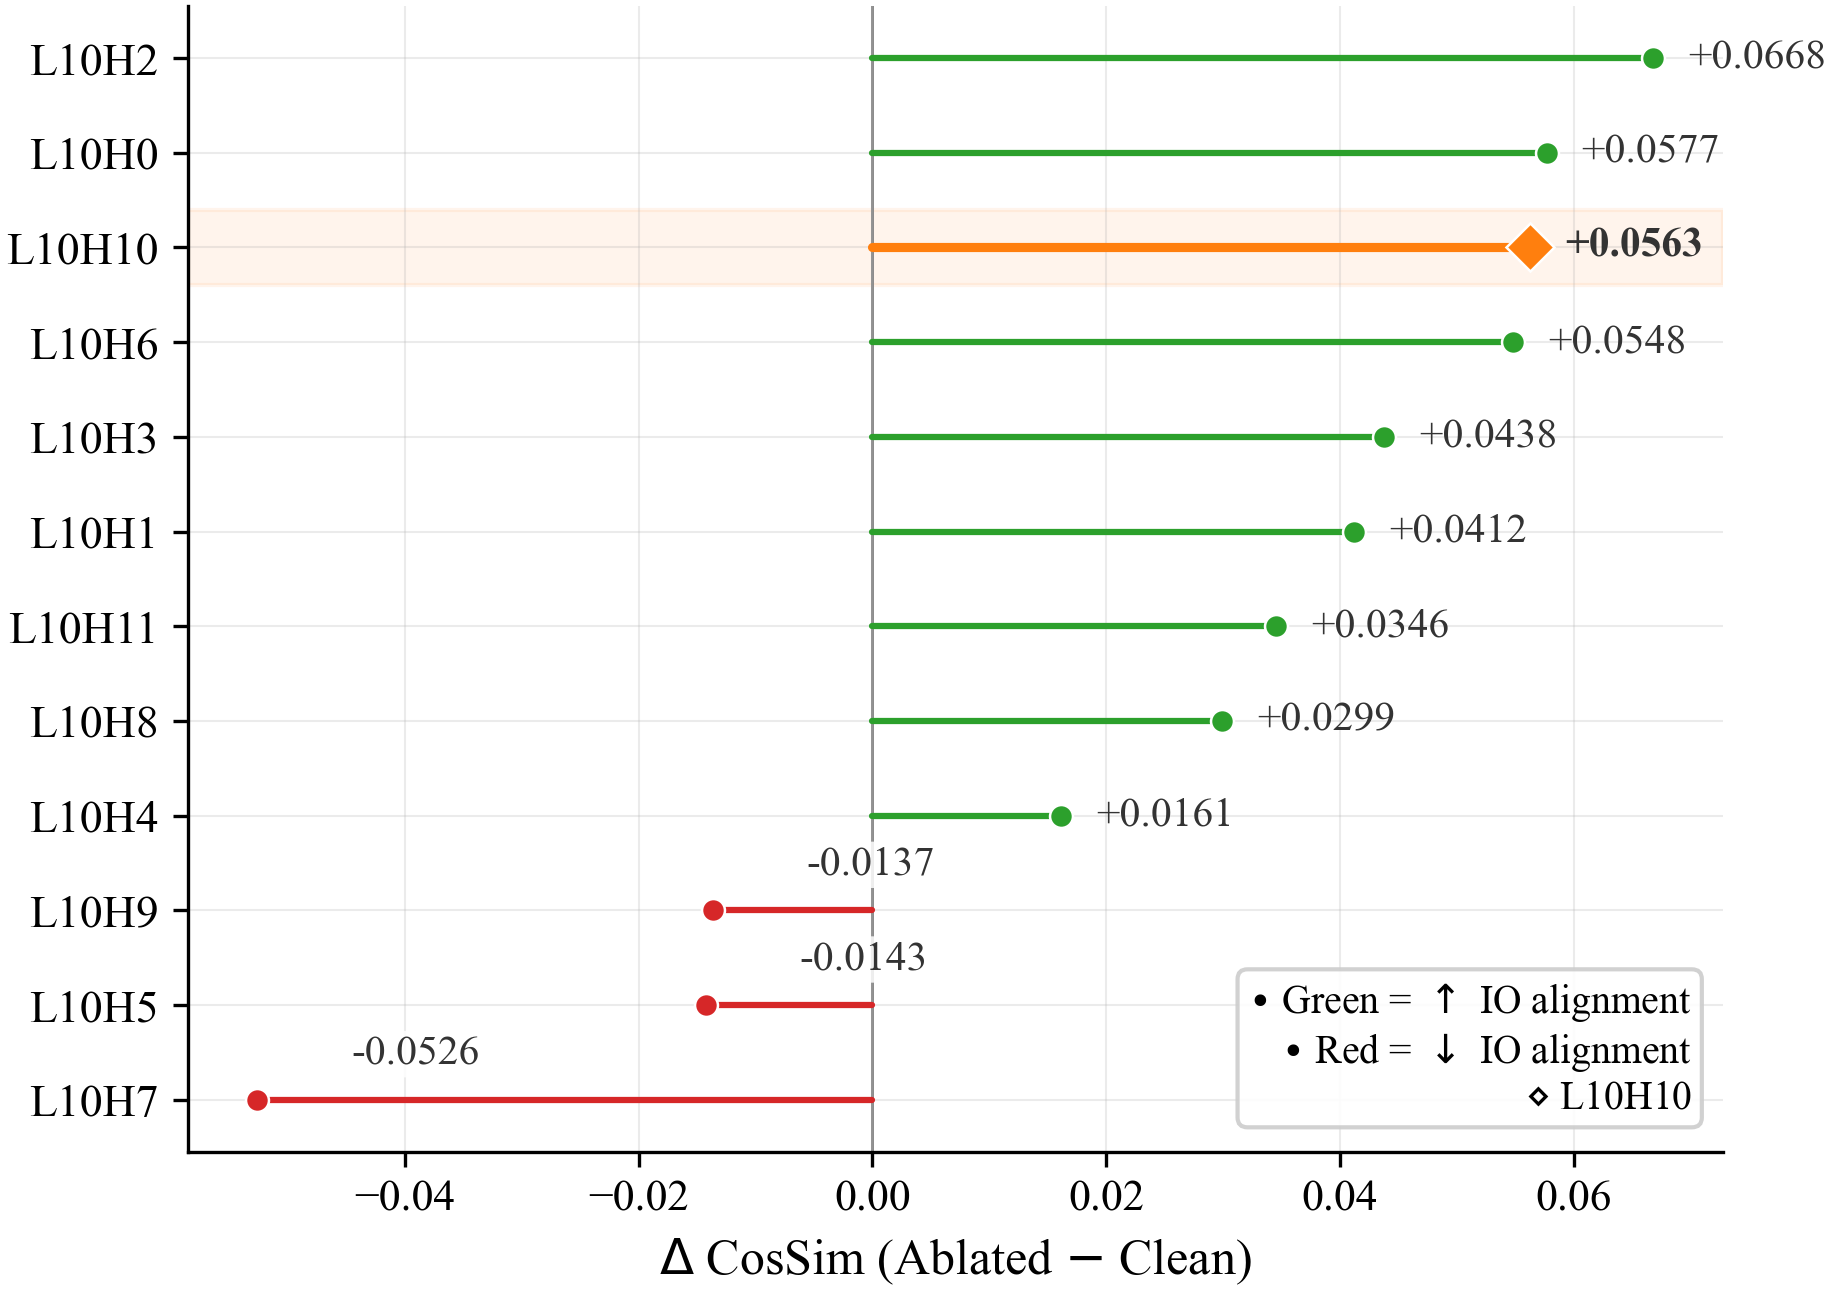
\includegraphics[width=0.92\linewidth]{figures/cossim_shift_lollipop.png}
  \caption{%
    \textbf{QK cosine similarity shifts across Layer 10 heads.}
    $\Delta_\text{CosSim}$ (ablated $-$ clean). Green/red: $\uparrow$/$\downarrow$ $IO$ alignment; L10H10 in orange.
  }
  \label{fig:cossim_shift}
\end{figure}

\begin{figure}[!htbp]
  \centering
  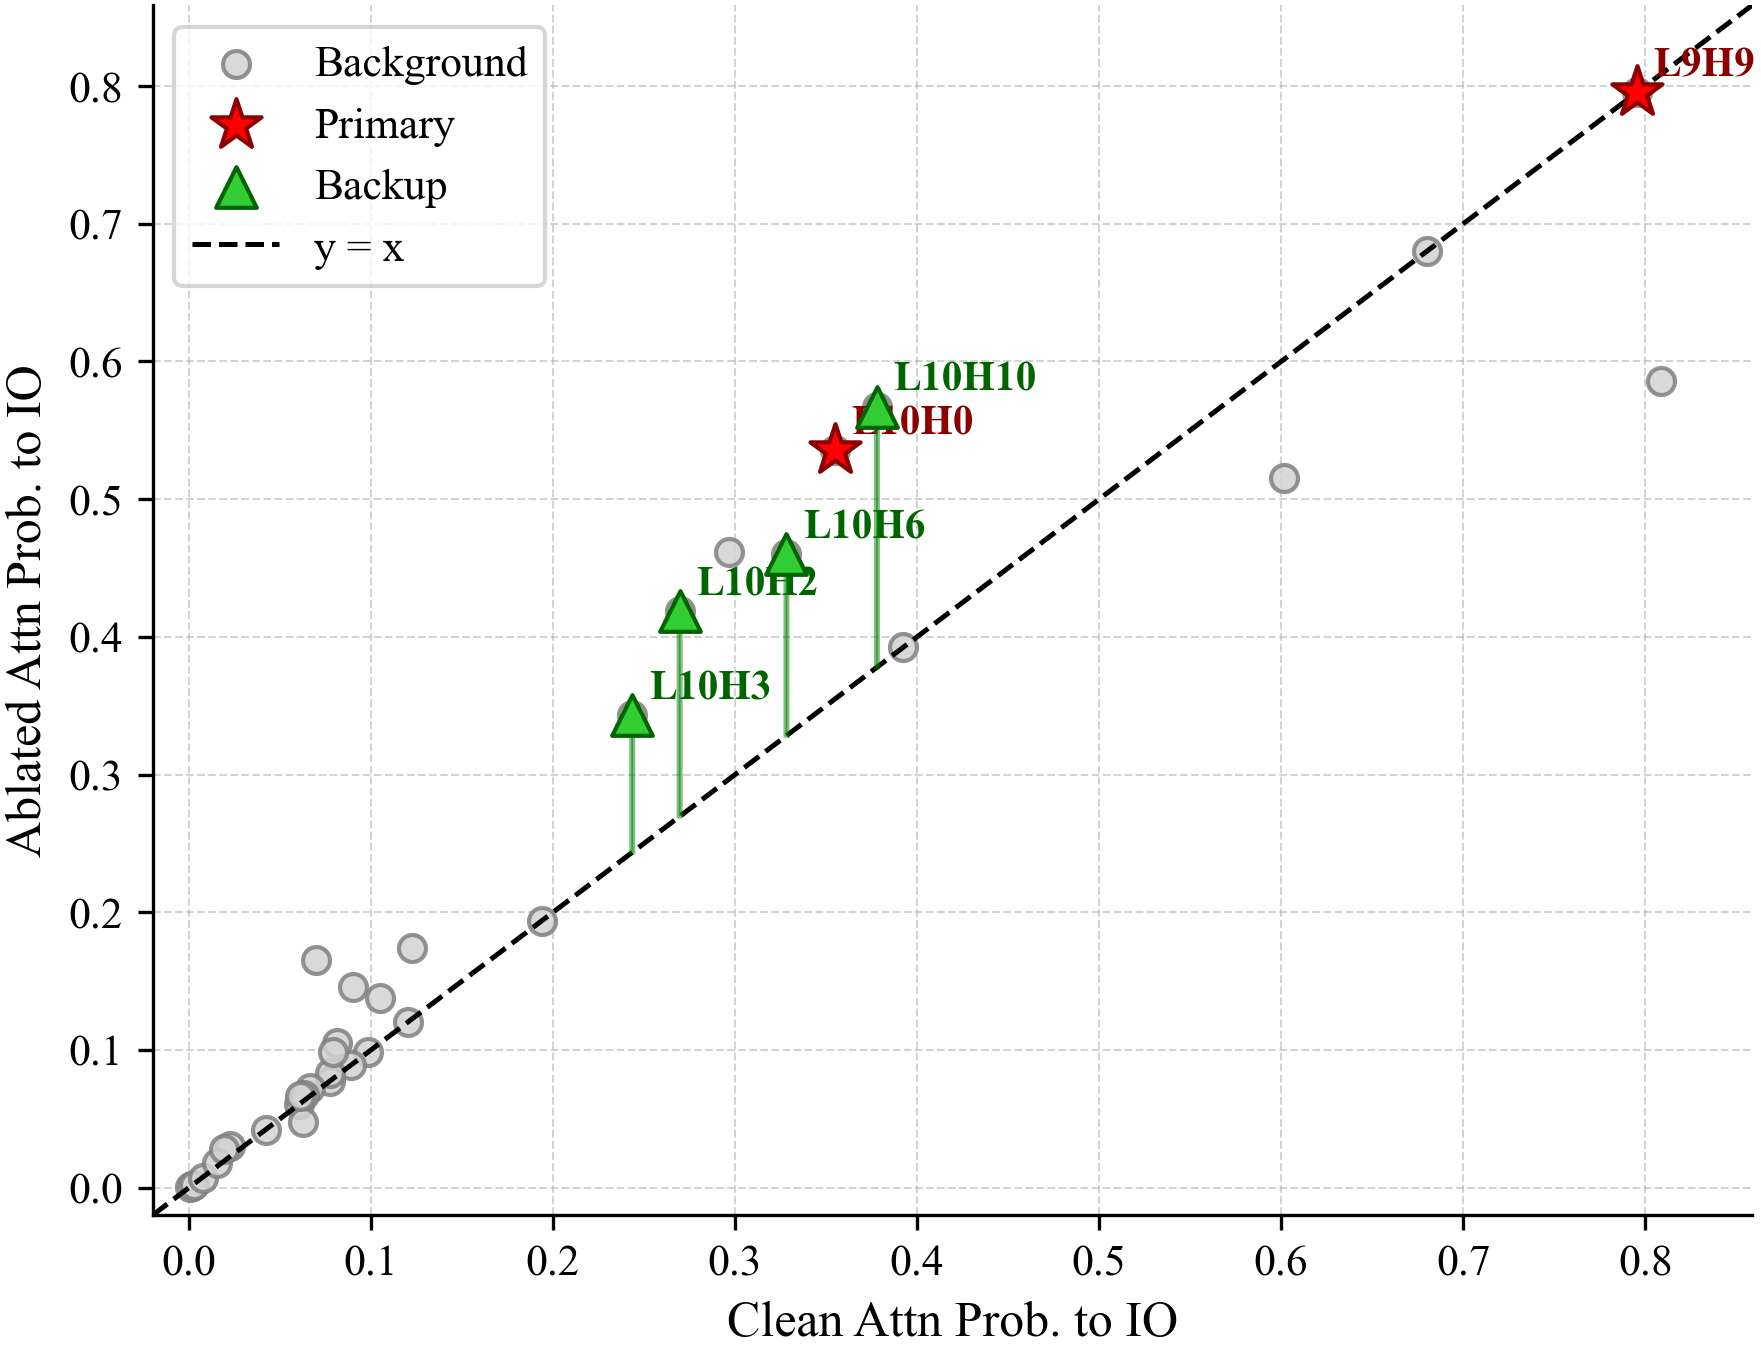
\includegraphics[width=0.92\linewidth]{figures/causal_shift_plot.png}
  \caption{%
    \textbf{Causal shift trajectory plot.}
    Clean vs.\ ablated $IO$ attention (Layer 9--11). Above $y=x$: Hydra spike.
  }
  \label{fig:causal_shift}
\end{figure}

\begin{figure}[!htbp]
  \centering
  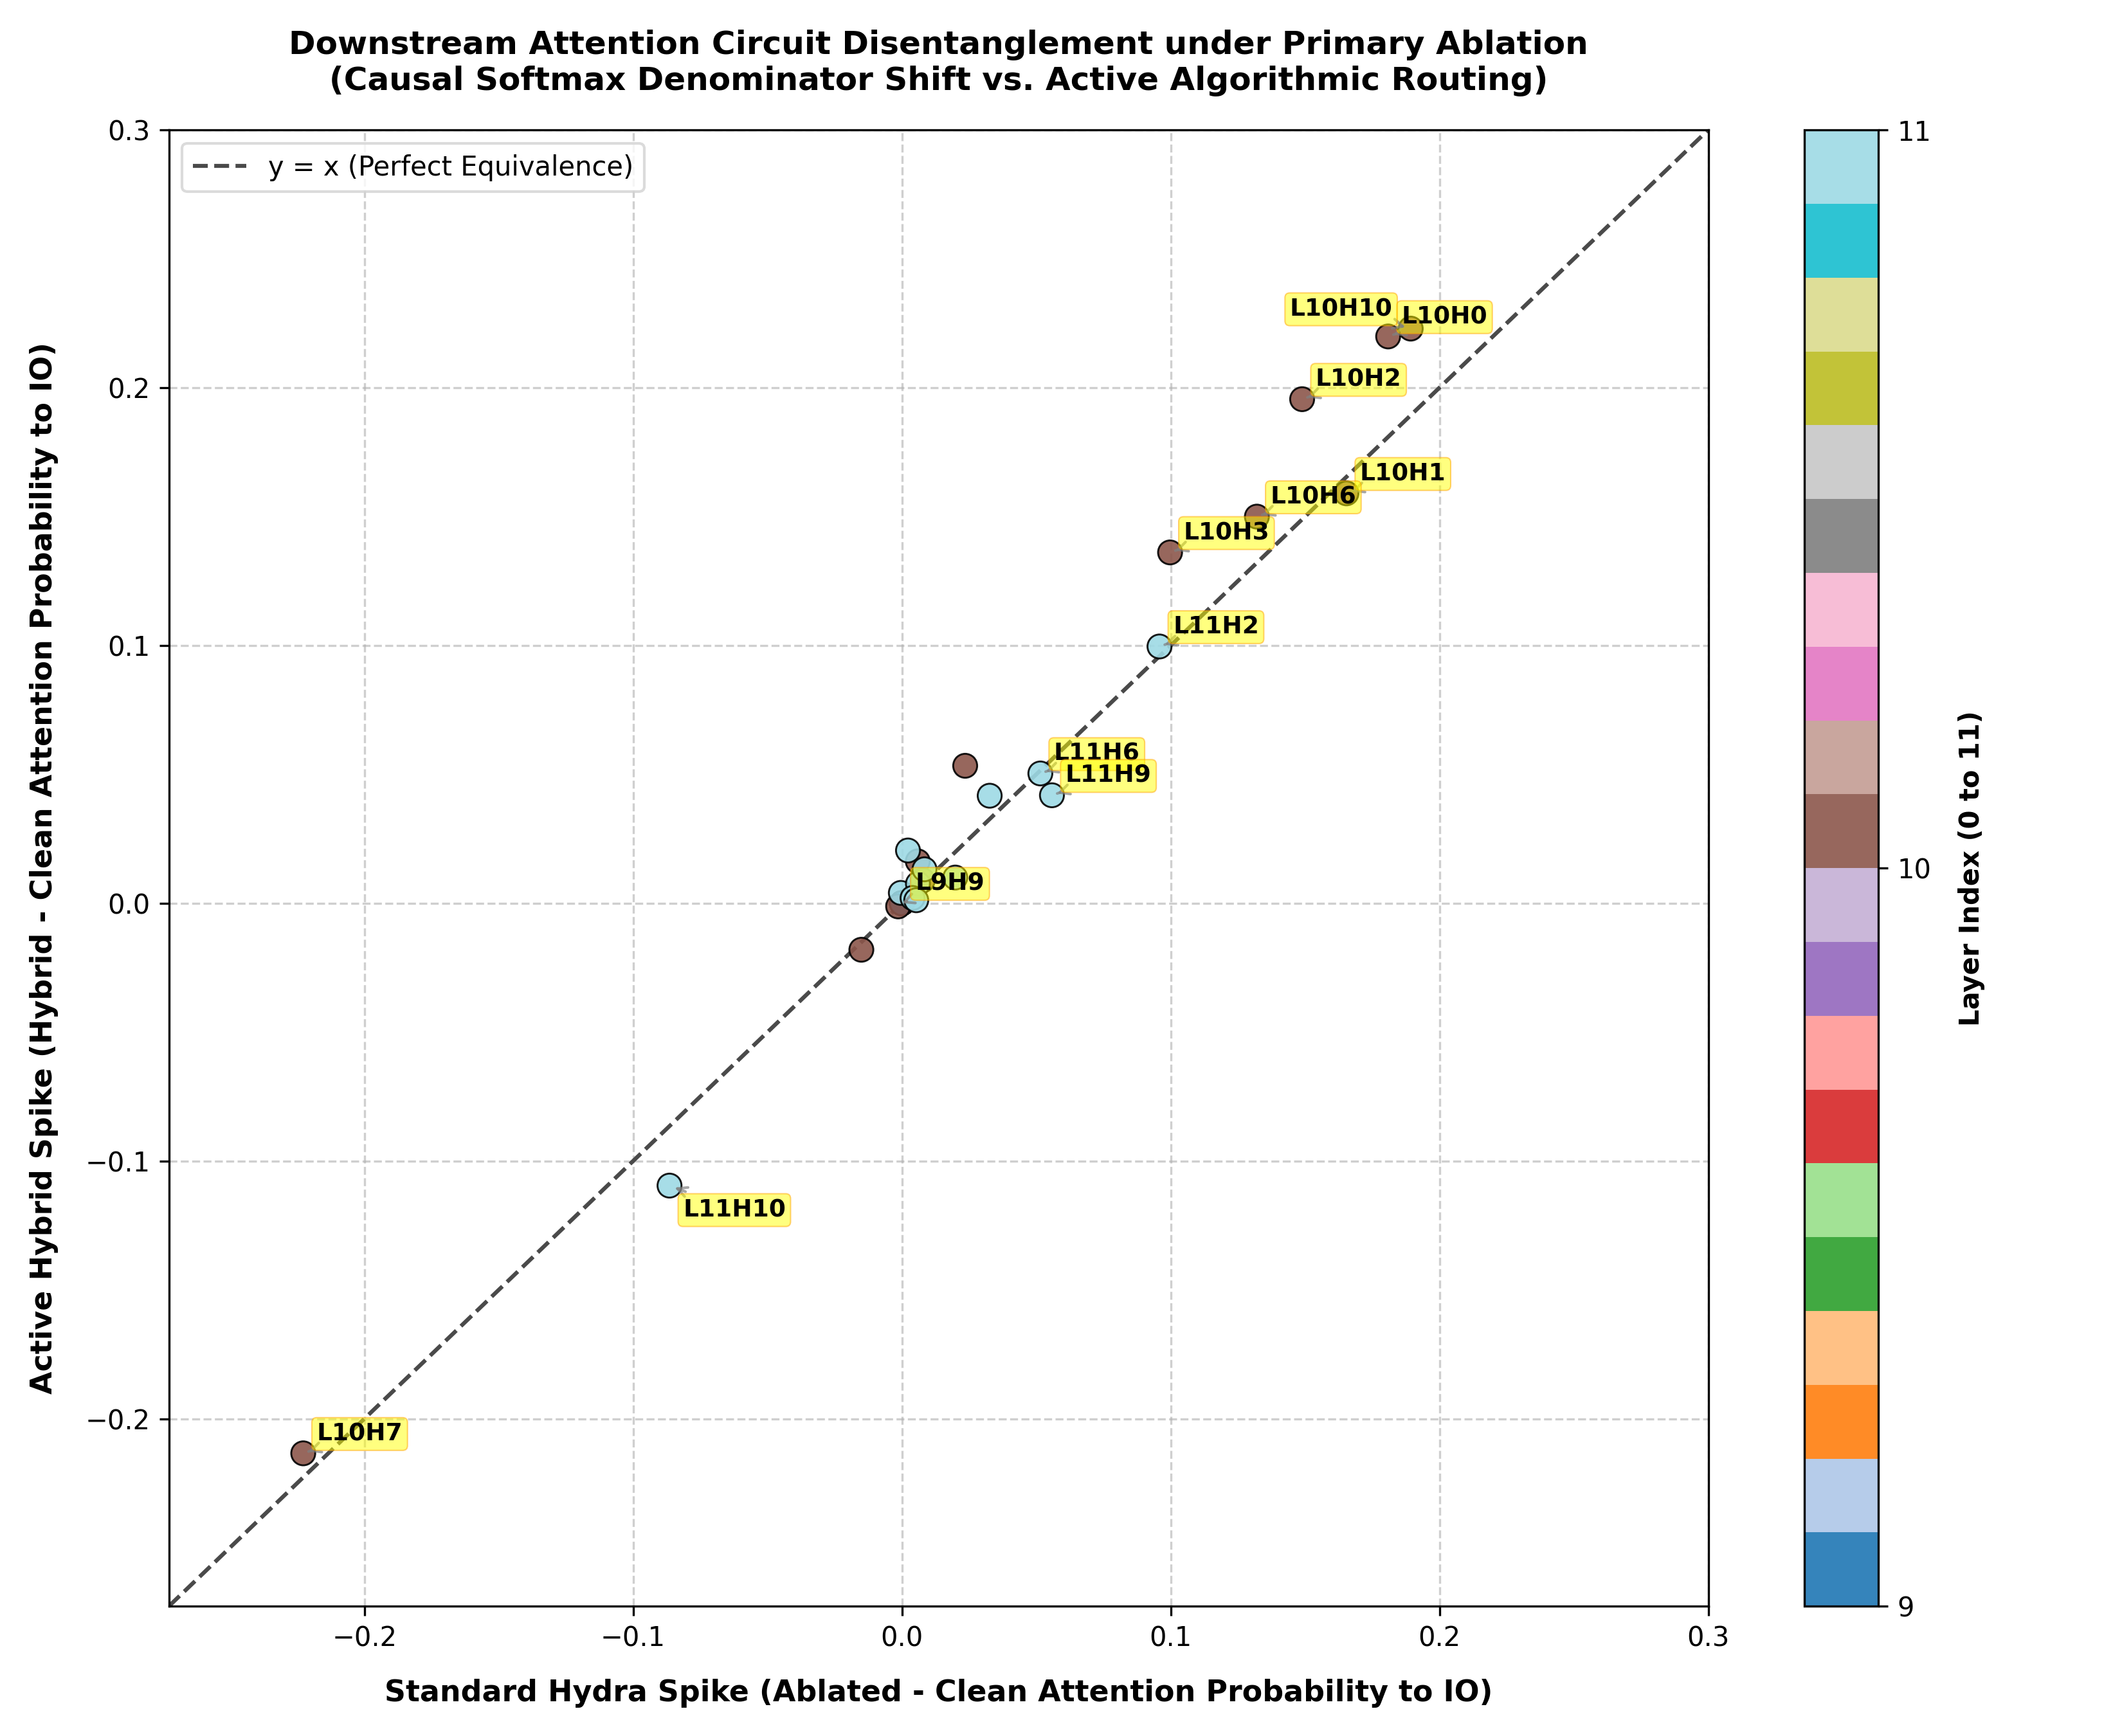
\includegraphics[width=0.92\linewidth]{figures/circuit_disentanglement_plot.png}
  \caption{%
    \textbf{FALI circuit disentanglement plot.}
    Standard spike vs.\ FALI target-logit contribution; above $y=x$ = underestimation.
  }
  \label{fig:disentanglement}
\end{figure}

\begin{figure}[!htbp]
  \centering
  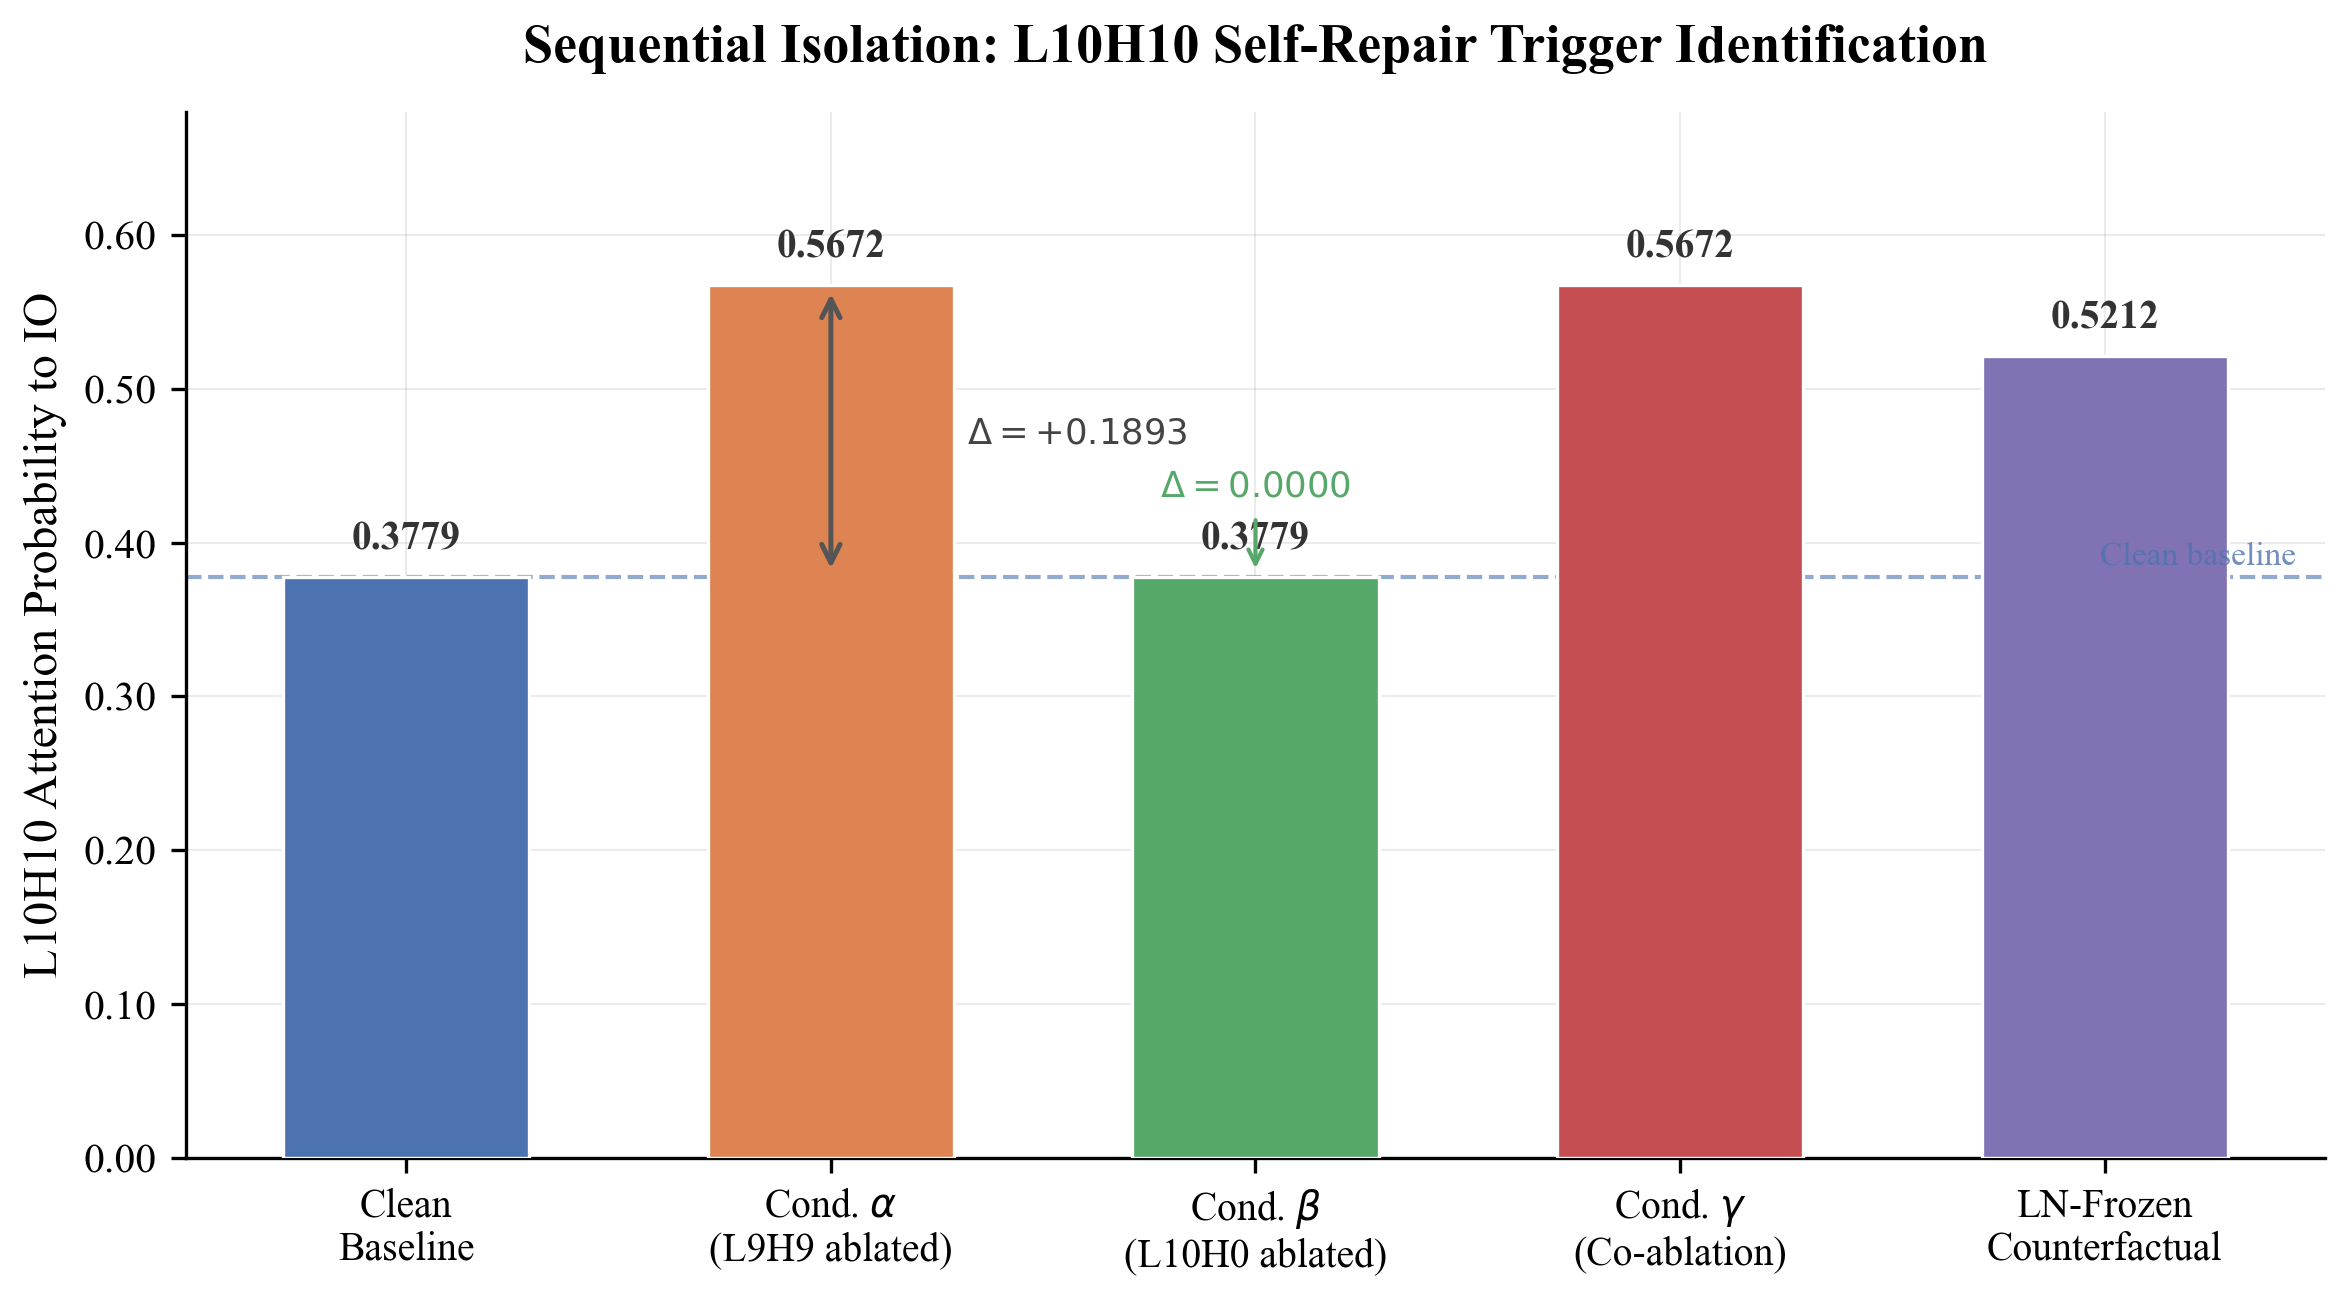
\includegraphics[width=0.92\linewidth]{figures/isolation_bar_chart.png}
  \caption{%
    \textbf{Sequential isolation of L10H10's self-repair trigger.}
    $\alpha$: $+0.1893$; $\beta$: $0$; LN-Frozen: $+0.1433$ (24.3\% removed).
  }
  \label{fig:isolation}
\end{figure}

\subsection{Ablation Control Analysis}
To verify that the observed attention spike and downstream compensation of the backup head L10H10 are realized routing effects rather than artifacts of a specific zero-ablation protocol, we compare the L10H10 response under zero, position-wise mean, and resampling ablation controls. Under zero ablation, the primary mover heads L9H9 and L10H0 are nullified, producing an L10H10 attention spike to the target token $IO$ of $+0.1893$ and an additional logit drop (causal degradation) of $0.2281$ when L10H10 is also ablated. Under position-wise mean ablation (where ablated activations are replaced by clean-run positional averages), the attention spike remains highly robust at $+0.1616$, and the causal degradation is $0.2048$. Under resampling ablation (where activations are resampled from a random cohort sample using a fixed derangement), the attention spike is $+0.1224$ and the causal degradation is $0.2435$. Across all three control paradigms, the attention spike is positive in $91.5\%$ to $100\%$ of cases, confirming that the self-repair signal is robust and survives under manifold-respecting ablation conditions.

\subsection{Path-Stable Attention Decomposition}
To understand whether L10H10's $+0.1893$ attention probability spike is driven by IO-target logit changes or background-logit shifts, we perform a path-stable, path-independent Shapley decomposition of the softmax probability delta. Under FALI, we isolate the pre-softmax attention logit matrix row. The total spike is $+0.1893$. Our Shapley decomposition shows that the target-logit pre-softmax score shift contributes $+0.2222$, accounting for $117.4\%$ of the total shift, while the background-logits shift contributes $-0.0328$, representing a negative fraction of $-17.4\%$. In $96.0\%$ of the IOI cohort samples, the background-logit contribution opposes the total spike, indicating that background-logit changes oppose the IO attention increase on average. Furthermore, the path-stability is extremely high, with an absolute target-background path disagreement of just $0.00153$ (a relative disagreement of $0.69\%$).

\subsection{Query-Key Geometry and Norm Decomposition}
To analyze what drives the target-logit score increase ($+0.9632$ score delta), we decompose the query and key vectors of L10H10 at the query position (\texttt{end}) and target key position ($IO$) into norm and directional/cosine alignment components. 
The total pre-softmax score delta is $+0.9632$. Applying Shapley decomposition to the high-dimensional QK representations reveals that:
\begin{itemize}
  \item \textbf{Query Vector Rotation}: The query vector shift yields a Query Shapley contribution of $+0.9770$, explaining $101.4\%$ of the score delta.
  \item \textbf{Key Vector Shift}: The key vector shift yields a Key Shapley contribution of $-0.0137$, representing a slight opposing effect ($-1.4\%$).
  \item \textbf{Directional/Cosine Alignment}: The change in directional cosine similarity yields a Cosine Shapley contribution of $+0.7418$, explaining $77.0\%$ of the score delta.
  \item \textbf{Norm Scaling}: The change in query-key norm product yields a Norm Shapley contribution of $+0.2214$, accounting for $23.0\%$ of the delta.
\end{itemize}
These results provide geometric evidence that the L10H10 IO-target score increase is primarily query-driven and largely cosine-alignment-driven, reflecting increased directional alignment in the QK representation space.

\subsection{Output-Level Causal Mediation}
Lastly, we evaluate whether L10H10's ablated-run activations causally mediate downstream $IO - S$ logit difference recovery. Clean baseline logit difference is $+2.9732$, primary ablation reduces it to $+2.1055$ (a degradation of $0.8677$), and double ablation (Pass C) further degrades performance to $+1.8775$ (a causal degradation of $0.2281$).
We run two targeted counterfactual path-patching interventions:
\begin{itemize}
  \item \textbf{Attention-Pattern Necessity}: Patching the clean attention pattern of L10H10 into the ablated model yields an aggregate pattern necessity effect of $0.0994$, causally explaining $43.6\%$ of the zero-ablation degradation.
  \item \textbf{$z$-Vector Output Necessity}: Patching the clean $z$-vector output of L10H10 into the ablated model yields an aggregate $z$ necessity effect of $0.1002$, causally explaining $44.0\%$ of the degradation.
\end{itemize}
In contrast, the low-effect control head L10H5 shows negligible pattern or $z$-vector necessity, while L10H2, L10H3, and L10H6 also show positive contributions. This supports L10H10 as one important contributor among several Layer 10 backup-like heads, rather than a uniformly replaceable effect across all heads.

% ===================================================================
\section{Discussion}
\label{sec:discussion}
% ===================================================================

\subsection{Why Layer 10? Semantic Representation Separation and Positional Readout}
\label{subsec:layer10}

The concentration of self-repair behavior in Layer 10 may reflect its position in the IOI circuit. In GPT-2 Small's IOI circuit, Layer 10 sits at a critical
juncture: it is the layer immediately following Layer 9, which houses the
dominant primary head (L9H9). By the time computation reaches Layer 10, the
residual stream has accumulated the full product of earlier layers' attention
and MLP transformations, and the semantic distinctions between $IO$ and $S$ may be especially accessible. Layer 10 heads may therefore have access to a favorable informational substrate for discriminating between the indirect object
and subject name tokens.

Furthermore, Layer 10 heads are positioned to directly read off the name mover
signal before it accumulates downstream through the final MLP layers
(Layers 10--11 MLP blocks). One possible explanation is that Layer 10 sits at a
favorable point in the IOI circuit, while later layers may have less separable
IO-vs-S information. Direct representational tests would be needed to verify this.

\subsection{Deconstructing the Intra-Layer Parallel Communication Hypothesis}
\label{subsec:isolation}

A major hypothesis in transformer self-repair literature posits that backup heads within a layer compensate directly in parallel for ablated primary heads in the same layer---the \emph{intra-layer parallel communication} hypothesis. Under this view, L10H10's attention spike would be a direct response to the ablation of its co-located Layer 10 partner, L10H0. 

To causally evaluate this hypothesis, we deconstructed the co-ablation protocol into three isolated sequential ablation runs across the 200-sample cohort:
\begin{itemize}
  \item \textbf{Condition $\alpha$ (Zero-ablate L9H9 only):} L10H10's attention to $IO$ spikes from a clean baseline of $0.3779$ to $0.5672$ ($\Delta = +0.1893$).
  \item \textbf{Condition $\beta$ (Zero-ablate L10H0 only):} L10H10's attention to $IO$ remains perfectly unchanged at $0.3779$ ($\Delta = 0.0000$).
  \item \textbf{Condition $\gamma$ (Co-ablation of both):} L10H10's attention to $IO$ spikes to $0.5672$ ($\Delta = +0.1893$).
\end{itemize}

These results show that L10H10's attention-pattern shift is triggered by upstream L9H9 ablation, not by same-layer L10H0 z-ablation. Because same-layer attention heads compute in parallel, the absence of a same-layer L10H0 z-ablation effect is partly architecturally expected. Under upstream primary-head ablation, L10H10 shows target-directed QK/logit changes consistent with compensatory routing. Specifically, L10H10 responds to the altered residual-stream state induced by upstream L9H9 ablation rather than same-layer L10H0 z-ablation, consistent with a cross-layer compensatory pathway in this intervention setup.

Figure~\ref{fig:isolation} visualizes L10H10's attention probability to $IO$ across all five experimental conditions. Condition $\beta$ (L10H0-only ablation) produces identically zero change from clean baseline, while Condition $\alpha$ (L9H9-only ablation) reproduces the full co-ablation spike ($+0.1893$). The LN-Frozen counterfactual bar (purple) shows the reduced delta ($+0.1433$) under the LayerNorm-scale freezing diagnostic, representing the scale-frozen component of the self-repair response.

\subsection{Softmax Bias as a Systematic Interpretability Confound}
\label{subsec:bias}

The FALI results reveal a systematic bias in standard ablation-based
interpretability methodology. The softmax function, while necessary for
producing valid probability distributions, introduces a non-local dependency:
the probability assigned to any token is a function of \emph{all} other tokens'
logits. When an ablation intervention changes the residual stream, it propagates
changes to all downstream heads' query and key projections via LayerNorm
amplification, which then affects \emph{all} pre-softmax logits in all downstream
heads, not only the logits directed toward the target token.

Standard causal ablation measures the total observed change in attention
probability, which conflates: (a) the change in the target token's logit due to
altered query-key alignment, and (b) the change in all non-target tokens' logits
due to LayerNorm volume surges. For heads where the LayerNorm surge reduces
the non-target logits more than it reduces the target logit (an asymmetric
effect that can arise when the non-target representations are more dependent on
the ablated head's signal), the net effect is an apparent increase in $IO$
attention probability even without any active change in the $IO$-directed logit.

This confound is particularly dangerous for the \emph{attribution} of functional
roles in circuit analysis. If L10H10's Hydra spike were merely a post-softmax redistribution artifact, then removing the head would not be expected to further degrade recovery, and its ablation would not further degrade model performance. Our
four-pass causal validation qualifies this response: Pass C
demonstrates that removing L10H10 after primary ablation causes an additional
10.83\% degradation in logit difference ($2.1055 \to 1.8775$), confirming that
the head's contribution is causal under the tested intervention and not merely an
epiphenomenal redistribution of normalization mass.

\subsection{Implications for Circuit Analysis Methodology}

Our findings have several methodological implications for the broader
mechanistic interpretability community:

\paragraph{1. Logit-level intervention strengthens head-level attribution.}
Attention-pattern analysis at the post-softmax level is insufficient to
distinguish target-logit from background-logit contributions. This is
consistent with recent work emphasizing that plausible circuit overlap or
component selection is not sufficient evidence of causal faithfulness
\citep{hanna2024faithfulness,gupta2024interpbench}. For responsive attention
heads, pre-softmax decomposition provides an additional validity check before
assigning a target-directed functional role.

\paragraph{2. LayerNorm must be treated as a first-order confound.}
The LayerNorm-mediated volume surge is not a second-order effect but a first-order
mechanism that modifies the absolute magnitude of all downstream attention logits.
Interpretability analyses that do not control for LayerNorm interactions
may systematically misattribute the sources of attention pattern changes.

\paragraph{3. LayerNorm scale drop represents a non-negligible confound.}
Across the prominent Layer 10 backup ensemble, standard ablation metrics overestimate the scale-frozen routing component by 17.8\% to 26.8\% (mean $\approx 22.8\%$) under the Layer-10 clean-scale intervention. However, the fact that a robust scale-frozen routing component remains under LayerNorm-scale freezing conditions, coupled with highly significant Query-Key spatial contraction, supports the presence of intervention-specific compensatory pathways in this model and task.

\paragraph{4. Standard causal tracing may misidentify ``important'' heads.}
If passive softmax artifacts can inflate the apparent Hydra response of
weakly-routed heads (e.g., L10H1 with $\rho \approx +3.8\%$), they could also
inflate the apparent importance of heads in other tasks where the LayerNorm
surge is more pronounced. FALI or analogous logit-level decomposition should be
applied as a validity check in circuit identification studies.

Conditional backup discovery and mechanism decomposition are complementary.
Conditional Co-Ablation identifies components whose importance emerges after
a primary circuit is disrupted \citep{gong2026conditional}; FALI analyzes
whether the resulting attention response is driven by the target token's logit
or by changes in competing logits. Applying both classes of methods could
separate three questions that are often conflated: which component becomes
necessary, what internal quantity changes, and whether that change causally
supports output recovery.

% ===================================================================
\section{Limitations}
\label{sec:limitations}

While our multi-method causal and geometric analysis provides robust evidence for backup self-repair under the tested primary-ablation intervention, several structural limitations bound the scope and generalizability of our findings:

\begin{enumerate}
  \item \textbf{Single Model Architecture:} The FALI experiments are conducted only on GPT-2 Small. Broader forms of self-repair and conditional backup activation have been observed across multiple model families and tasks \citep{rushing2024selfrepair,gong2026conditional}, but the specific target-versus-background FALI decomposition, QK mechanism, and mediation fractions reported here have not been validated beyond GPT-2 Small IOI.
  \item \textbf{Single Task and Dataset Cohort:} Our circuit analysis is restricted to the name-copying circuit of the Indirect Object Identification (IOI) task family, evaluated on an $N=200$ mixed-template cohort. Testing on other sequence benchmarks (e.g., factual recall, modular arithmetic, translation) is required to generalize the circuit dynamics.
  \item \textbf{Targeted Primary Ablation:} Our interventions focus specifically on the ablation of the primary name mover heads \texttt{L9H9} and \texttt{L10H0}. While zero, position-wise mean, and resampling ablation controls confirm that the self-repair signal is not a zero-ablation-specific anomaly, these controls do not mathematically establish a general backup mechanism across arbitrary component failures.
  \item \textbf{Interpretive Boundary of FALI:} FALI is a controlled logit-level decomposition that isolates the IO-target attention-logit contribution from background-logit contributions. However, because attention logits arise from coupled Query-Key geometry, background-logit changes may themselves be downstream consequences of the same ablation-induced representational shift that increases the target logit. FALI should therefore be viewed as a diagnostic for target-specific routing and denominator effects, not as a complete separation of all active and passive mechanisms.
  \item \textbf{Intervention Specificity:} Our causal claims are tied to the specific hook-patching configurations implemented. While we verify that the ablated-run activations of \texttt{L10H10} explain $44.0\%$ of its zero-ablation degradation by aggregate ratio of means, the remaining degradation may be mediated by other heads or paths that were not concurrently isolated.
  \item \textbf{Semantic Content of Backup Signals:} The $z$-patching result shows that L10H10's head output is causally relevant to downstream recovery under the tested intervention, explaining $44.0\%$ of L10H10's zero-ablation degradation by aggregate ratio of means. However, we have not yet performed direct Value ($V$) or Output-Value ($OV$) path patching. Consequently, while we establish an output-level causal contribution, the specific semantic content of the written signal---such as name-copying features versus generic positional or token-selection features---remains partially uncharacterized.
\end{enumerate}

Table~\ref{tab:claims_evidence} presents a summary of our primary research claims, their key causal evidence, empirical strength, and structural limitations.

\begin{table}[t]
  \centering
  \caption{Claims, causal evidence, and strength matrix}
  \label{tab:claims_evidence}
  \scriptsize
  \resizebox{\linewidth}{!}{%
  \begin{tabular}{lp{4.6cm}ll}
    \toprule
    \textbf{Claim} & \textbf{Key Causal Evidence} & \textbf{Strength} & \textbf{Limitation} \\
    \midrule
    \textbf{Robust Attention Spike} & L10H10 attention spike is robust across zero ($+0.1893$), mean ($+0.1616$), and resample ($+0.1224$) ablations ($91.5\%$--$100\%$ positive). & Strong in this setting & $N=200$ cohort size. \\
    \textbf{Target-Logit Dominance} & Shapley shows target pre-softmax shift is $+0.2222$ ($117.4\%$ fraction); background opposes shift in $96.0\%$ of samples ($-17.4\%$ fraction). & Strong in this setting & Alignment-dependent. \\
    \textbf{Query-Driven Alignment} & QK delta ($+0.9632$) is driven by query rotation ($+0.9770$ / $101.4\%$) and directional cosine alignment increase ($+0.7418$ / $77.0\%$). & Strong in this setting & Invariant to value path. \\
    \textbf{Causal Downstream Rescue} & Double ablation causes $0.2281$ logit drop. L10H10 pattern/z necessity explain $43.6\%$ / $44.0\%$ of the degradation; L10H2, L10H3, and L10H6 are additional contributing Layer 10 heads; L10H5 is a low-effect control; L10H7 is anti-backup/suppressor-like under this intervention. & Strong & No direct V/OV path patching. \\
    \textbf{Cross-Layer Trigger} & Upstream L9H9 ablation alone triggers full L10H10 spike ($+0.1893$); intra-layer L10H0 ablation produces zero shift ($0.0000$). & Strong in this setting & Task-specific pathway. \\
    \bottomrule
  \end{tabular}%
  }
\end{table}

% ===================================================================
\section{Conclusion}
\label{sec:conclusion}
% ===================================================================

We have presented the \textbf{Frozen Attention Logit Intervention (FALI)}, a
novel mechanistic intervention that surgically decomposes the Hydra Effect into
its target-logit and background-logit pre-softmax attention contributions. Applied
to GPT-2 Small on the IOI benchmark with a cohort of 200 samples across all 144
attention heads, our method yields several principal findings that outline a structured result chain:

\begin{enumerate}
  \item \textbf{Ablation controls verify the robustness of the backup response.} Zero, position-wise mean, and resampling ablation controls confirm that L10H10's attention probability spike is not a zero-ablation-specific anomaly but survives under manifold-respecting ablation conditions.

  \item \textbf{Target-logit attention contributions dominate in the Layer 10 backup ensemble.} Shapley decomposition reveals that L10H10's $+0.1893$ attention spike is dominated by the IO-target attention-logit contribution ($+0.2222$), while background-logit changes oppose the spike on average in $96.0\%$ of samples ($-17.4\%$ fraction).

  \item \textbf{Query-driven and cosine-alignment-driven mechanisms shape the representation geometry.} Cosine similarity tracking ($p = 2.32 \times 10^{-109}$) and QK decomposition show that this pre-softmax score increase is primarily query-driven and largely cosine-alignment-driven, reflecting targeted spatial realignment in the attention manifold.

  \item \textbf{L10H10 causally contributes to recovery under the tested primary-ablation intervention.} Four-pass causal validation shows that L10H10's attention-pattern change causally contributes to downstream $IO - S$ logit recovery under the tested primary-ablation intervention, explaining about $43.6\%$ of the zero-ablation degradation under pattern necessity. The head's isolation ablation (Pass D, $-7.98\%$ from clean baseline) confirms its role as a context-sensitive backup rather than a primary processor.
\end{enumerate}

Separately, our LayerNorm-scale freezing diagnostics separate denominator scaling from logit routing: under the Layer-10 clean-scale intervention, 24.3\% of the observed L10H10 attention spike is removed (reducing the attention probability shift from $+0.1893$ to $+0.1433$). This confirms that LayerNorm scale changes systematically inflate standard metrics across the Layer 10 backup ensemble by 17.8\% to 26.8\% (mean $\approx 22.8\%$), showing that LayerNorm surges represent important, non-negligible scale confounds that should be controlled for as a separate diagnostic.

Together, these results support a refined perspective in how transformer
self-repair should be conceptualized: the tested backup heads include target-directed
attention-logit changes that cannot be explained by softmax normalization alone,
whose true computational contribution has been systematically
obscured by the non-local coupling introduced by the softmax denominator. The FALI framework provides a principled methodology for diagnosing softmax-induced bias in attention-pattern interpretation. While our empirical findings are currently limited to the IOI circuit in GPT-2 Small, the consistency of target-logit dominance across the Layer 10 ensemble suggests that FALI, or analogous pre-softmax decomposition methods, can serve as useful validity checks in circuit analysis for distinguishing target-directed attention-logit changes from normalization and denominator artifacts.

Future work should extend FALI to: (1) other tasks and model architectures
(e.g., Pythia, Gemma, LLaMA) to assess the generality of this backup mechanism;
(2) direct Value (V) and Output-Value (OV) path patching to characterize the
semantic content of the written backup signals; (3) gradient-based attribution
methods (e.g., attribution patching \citep{nanda2023attribution}) to provide a
computationally efficient approximation of FALI at scale.

% ===================================================================


% Fit the reference list on the preceding page (avoid a near-empty final page).
\setlength{\bibsep}{1.5pt plus 0.5pt minus 0.5pt}
{\small
\bibliographystyle{tmlr}
\bibliography{references}
}

\end{document}
